\chapter{Graph Coloring}
Rishnak was impressed with Ajur's logical reasoning ability and went searching for him. It did not take long for Rishnak to find him---ghosts can move rather quickly. He found Ajur and Jura sitting on a stone bench. Without hesitation, Rishnak asked Ajur if he liked coloring.

Ajur enthusiastically responded that he did indeed like to color and enjoyed its calming effect.

Rishnak was pleased with this response and introduced the next topic. He said, ``Let's talk today about graph coloring. A proper \textit{vertex coloring} of a graph is a coloring of vertices such that no adjacent vertices---I mean vertices connected by an edge---have the same color.''

Rishnak flashed his hands and a graph appeared in front of Ajur, but this graph gleamed with different colors [Figure~\ref{10g1}]. He said, ``This is an example of a proper vertex coloring of a graph using four colors.''

Ajur marveled at the graph in front of him.

\begin{figure}[ht]
\begin{center}
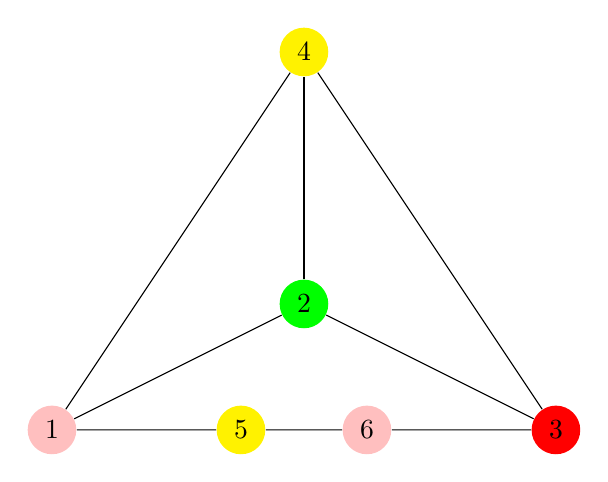
\begin{tikzpicture}
  [scale=.8,auto=left,every node/.style={circle}]
  \node (n1)[fill=pink] at (-1,7) {1};
  \node (n2)[fill=green] at (3,9)  {2};
  \node (n3)[fill=red] at (7,7)  {3};
  \node (n4)[fill=yellow] at (3,13)  {4};
  \node (n5)[fill=yellow] at (2,7) {5};
  \node (n6)[fill=pink] at (4,7) {6};
 \foreach \from/\to in {n1/n2,n2/n3,n2/n4,n1/n4,n3/n4,n1/n5,n5/n6,n6/n3}
    \draw (\from) -- (\to);
\end{tikzpicture}
\caption{A proper coloring of the vertices of a graph using four colors}\label{10g1}
\end{center}
\end{figure}

\begin{figure}[ht]
\begin{center}
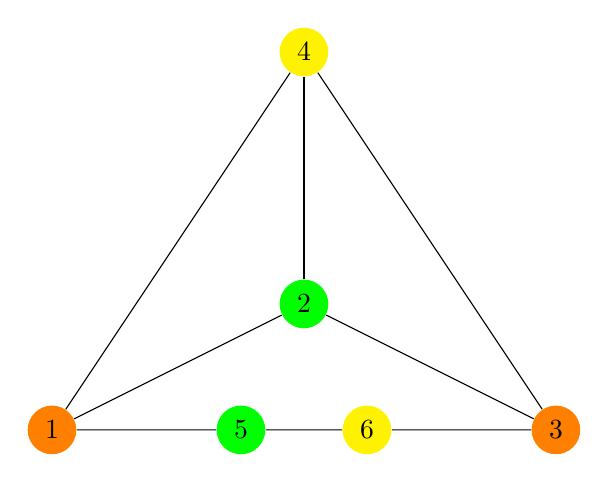
\begin{tikzpicture}
  [scale=.8,auto=left,every node/.style={circle}]
  \node (n1)[fill=orange] at (-1,7) {1};
  \node (n2)[fill=green] at (3,9)  {2};
  \node (n3)[fill=orange] at (7,7)  {3};
  \node (n4)[fill=yellow] at (3,13)  {4};
  \node (n5)[fill=green] at (2,7) {5};
  \node (n6)[fill=yellow] at (4,7) {6};
 \foreach \from/\to in {n1/n2,n2/n3,n2/n4,n1/n4,n3/n4,n1/n5,n5/n6,n6/n3}
    \draw (\from) -- (\to);
\end{tikzpicture}
\caption{A proper coloring of the vertices of the graph shown in Figure~\ref{10g1} using only three colors}\label{10g2}
\end{center}
\end{figure}

\begin{figure}
\begin{center}
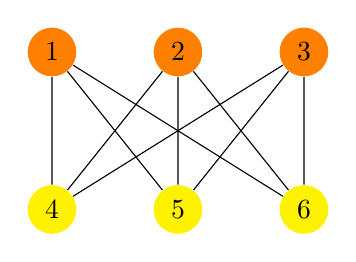
\begin{tikzpicture}
  [scale=.4,auto=left,every node/.style={circle}]
  \node (n1)[fill=orange] at (1,7) {1};
  \node (n2)[fill=orange] at (5,7)  {2};
  \node (n3)[fill=orange] at (9,7) {3};
  \node (n4) [fill=yellow] at (1,2)  {4};
  \node (n5) [fill=yellow] at (5,2) {5};
  \node (n6)[fill=yellow] at (9,2)  {6};

   \foreach \from/\to in {n1/n6,n1/n4,n1/n5,n2/n6,n2/n4,n2/n5,n3/n4,n3/n5,n3/n6}
    \draw (\from) -- (\to);
    \end{tikzpicture}
\caption{Two coloring of complete bipartite graph~$K_{3,3}$ with six vertices and nine edges}\label{10g3}
\end{center}
\end{figure}

Rishnak continued, ``An interesting problem is to determine the smallest number of colors to properly vertex color a graph. Can you do better than four colors for this graph, Ajur?''

Ajur jumped up from the stone bench and grabbed a stick. He said, ``Yes, I already see one with three colors.'' He drew a new graph in the dirt, using fallen leaves to show the three different colors [Figure~\ref{10g2}].

Rishnak asked, ``How do you know three is the minimum number of colors that you need for that graph?''

Ajur thought for a moment, then said, ``Three colors are needed because vertices~1, 2, and~4 are mutually adjacent, so those vertices need three distinct colors.''

Rishnak smiled and asked Ajur to properly color complete bipartite graph~$K_{3,3}$.

Ajur jumped at the opportunity and quickly drew graph~$K_{3,3}$ in the dirt, then used orange and yellow leaves to color the graph [Figure~\ref{10g3}].

Rishnak said, ``Good. How did you come to that answer so quickly?''

Ajur said, ``In a bipartite graph, vertices are partitioned into two sets~$A$ and~$B$. Since the edges always go from a vertex in~$A$ to a vertex in~$B$, all of the vertices in~$A$ can be colored with one color, say orange, while all of the vertices in~$B$ can be colored with another color, say yellow.''

Rishnak said, ``Right, and since you are using leaves, let's talk about trees. Since all trees are also bipartite graphs, trees can always be colored with just two colors.'' Rishnak waved his hands and a brightly colored red and pink graph appeared in front of Ajur [Figure~\ref{10g4}].

\begin{figure}
\begin{center}

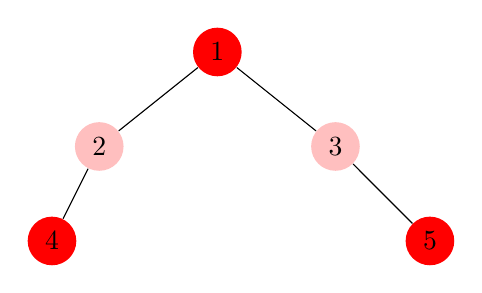
\begin{tikzpicture}
  [scale=.6,auto=left,every node/.style={circle}]
  \node (n1)[fill=red] at (5.5,7) {1};
  \node (n2)[fill=pink] at (3,5)  {2};
  \node (n3)[fill=pink] at (8,5)  {3};
  \node (n4)[fill=red] at (2,3) {4};
  \node (n5)[fill=red] at (10,3)  {5};


  \foreach \from/\to in {n1/n2,n1/n3,n2/n4,n3/n5}
    \draw (\from) -- (\to);

\end{tikzpicture}

\caption{Two coloring of a tree}\label{10g4}
\end{center}
\end{figure}

Ajur grew more curious and asked, ``Can you also color edges? And if so, is there a concept of adjacent edges?''

Rishnak always believed that asking the right questions is important because it is a signal that one's understanding is deepening. He responded, ``Yes, two edges are adjacent if they are incident to the same vertex. Consider this graph''---he waved his hands and a new graph appeared [Figure~\ref{10g5}]---``Edge~$e_1$ is adjacent to edge~$e_2$ since both are incident at vertex~1. Edge~$e_1$ is also adjacent to edges~$e_3$, $e_4$, and~$e_5$ because all of these edges are incident at vertex~2.''

\begin{figure}
\begin{center}

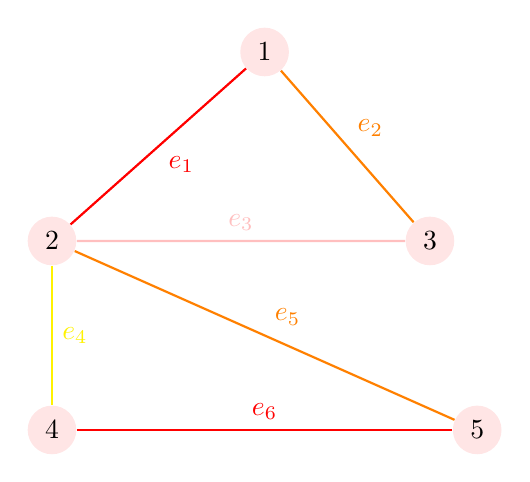
\begin{tikzpicture}
  [scale=.6,auto=left,every node/.style={circle,fill=red!10}]
  \node (n1) at (5.5,9) {1};
  \node (n2) at (1,5)  {2};
  \node (n3) at (9,5)  {3};
  \node (n4) at (1,1) {4};
  \node (n5) at (10,1)  {5};

\path[-,draw,thick,every node/.style={fill=none}]
    (n1) edge [color=red] node {$e_1$} (n2)
    (n1) edge [color=orange] node {$e_2$} (n3)
    (n2) edge [color=pink] node {$e_3$} (n3)
    (n2) edge [color=yellow] node {$e_4$} (n4)
    (n2) edge [color=orange] node {$e_5$}  (n5)
    (n4) edge [color=red]node {$e_6$}  (n5)
    ;

\end{tikzpicture}

\caption{Four edge coloring of a graph}\label{10g5}
\end{center}
\end{figure}

Ajur exclaimed, ``Then the maximum degree of this graph, which is four, tells us that we need four colors for the edge covering.''

Rishnak smiled and said, ``Your observation regarding the maximum degree of a graph is good, but the maximum degree of graph, call it~$\Delta$, does not imply that the graph has a~$\Delta$-coloring. Think of this graph''--Rishnak waved his hands and a new graph appeared [Figure~\ref{10g6}]--``and notice that it is a cycle of length~5 with a maximum degree of~$\Delta=2$, but it needs three colors to color its edges.''

\begin{figure}
\begin{center}

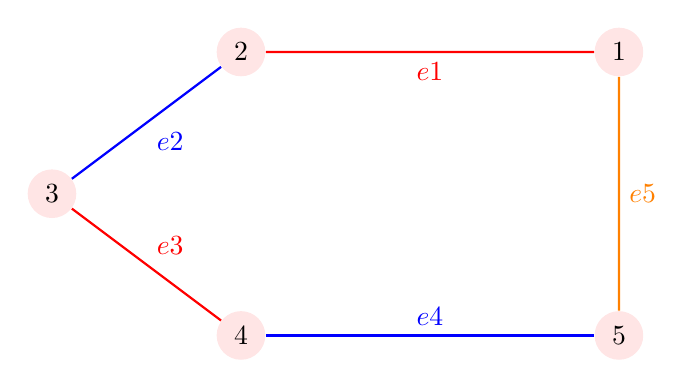
\begin{tikzpicture}
  [scale=.6,auto=left,every node/.style={circle, fill=red!10}]
  \node (n1) at (10,9) {1};
  \node (n2) at (2,9)  {2};
  \node (n3) at (-2,6)  {3};
  \node (n4) at (2,3) {4};
  \node (n5) at (10,3)  {5};

\path[-,draw,thick,every node/.style={fill=none}]
    (n1) edge [color=red] node {$e1$} (n2)
    (n2) edge [color=blue] node {$e2$} (n3)
    (n3) edge [color=red] node {$e3$} (n4)
    (n4) edge [color=blue] node {$e4$} (n5)
    (n1) edge [color=orange] node {$e5$}  (n5)
;
\end{tikzpicture}

\caption{Three edge coloring of a cycle of length~5}\label{10g6}
\end{center}
\end{figure}

Ajur frowned and said, ``Oh right, I see. I was hoping there was a simple mathematical explanation here.''

Rishnak said, ``There is. A graph with maximum degree~$\Delta$ can be edge colored with either~$\Delta$ or~$\Delta+1$ colors.''

Ajur's frown turned into a smile.

Rishnak also smiled, then said, ``A regular graph with degree~3---meaning a graph with all of its vertices having a degree of~3, also known as a \textit{trivalent graph}---that needs four edge colors for a proper edge coloring is known as a~\textit{Snark}.''

Ajur laughed. He had heard of Snarks from a poem titled \textit{The Hunting of the Snarks} by his dad's favorite author, Lewis Carroll.

Rishnak smiled and said, ``Strange name, yes, but graph theorists often have a whimsical sense of humor, and since four-edge-colorable trivalent graphs are awfully elusive, they named these graphs Snarks.''

Ajur thought for a moment, curious to find one for himself. He asked, ``Is the Petersen graph a Snark?''

Surprised that Ajur remembered, Rishnak replied that the Petersen graph indeed needs four colors to properly color the edges of that graph. He waved his hands and the graph appeared in front of Ajur [Figure~\ref{10g7}].

\begin{figure}
\begin{center}
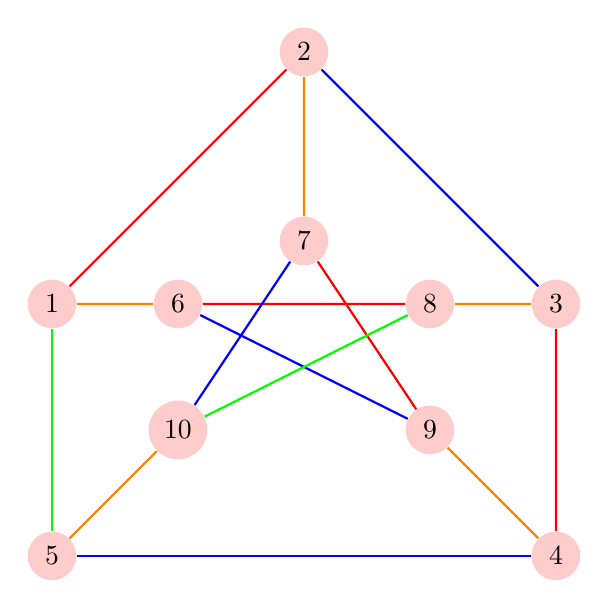
\begin{tikzpicture}
  [scale=.8,auto=left,every node/.style={circle,fill=red!20}]
  \node (n1) at (1,7) {1};
  \node (n2) at (5,11)  {2};
  \node (n3) at (9,7)  {3};
  \node (n4) at (9,3) {4};
  \node (n5) at (1,3) {5};
  \node (n6) at (3,7)  {6};
  \node (n7) at (5,8) {7};
  \node (n8)  at (7,7) {8};
  \node (n9) at (7,5) {9};
  \node (n10) at  (3,5) {10};
 \path[-,draw,thick]
    (n1) edge [color=red]  (n2)
    (n2) edge [color=blue]   (n3)
    (n3) edge [color=red]  (n4)
    (n4) edge [color=blue]  (n5)
    (n1) edge [color=green]  (n5)
    (n7) edge [color=red]   (n9)
    (n9) edge [color=blue]   (n6)
    (n6) edge [color=red]  (n8)
    (n8) edge [color=green]   (n10)
    (n10) edge [color=blue]  (n7)
    (n1) edge [color=orange] (n6)
    (n2) edge [color=orange] (n7)
    (n3) edge [color=orange] (n8)
    (n4) edge [color=orange] (n9)
    (n5) edge [color=orange] (n10)
    ;

\end{tikzpicture}
\caption{Four edge coloring of the Petersen graph, a regular graph of degree~3, and therefore a Snark}\label{10g7}
\end{center}
\end{figure}

Rishnak said, ``We can also convert an edge coloring problem to a vertex coloring problem. From a given graph~$G$ for which you want to color the edges, we can construct a new graph~$H$ in which edges of~$G$ become vertices of~$H$, and two vertices of~$H$ are adjacent if the corresponding edges in~$G$ are incident on the same vertex of~$G$.''

Rishnak flashed his hands and said, ``Here, let me show you.  The edge coloring of this graph''---he waved his hands and a previous graph appeared [Figure~\ref{10g5}]---``can be converted into a vertex coloring in this graph''---Rishnak waved his hands again and a new graph appeared [Figure~\ref{10g55}].

\begin{figure}
\begin{center}

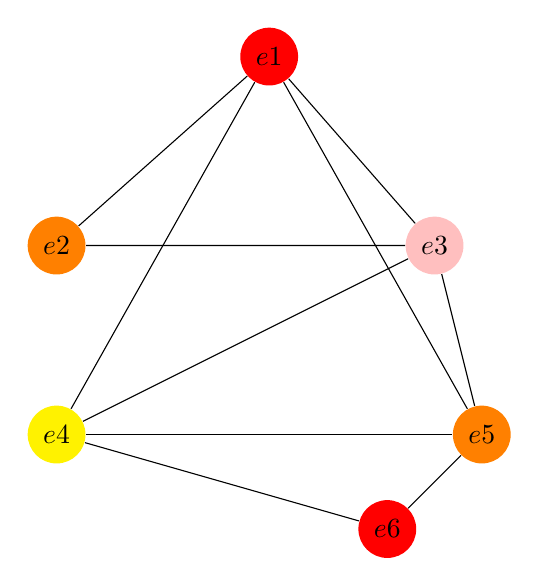
\begin{tikzpicture}
  [scale=.6,auto=left,every node/.style={circle}]
  \node (n1)[fill=red] at (5.5,9) {$e1$};
  \node (n2)[fill=orange] at (1,5)  {$e2$};
  \node (n3)[fill=pink] at (9,5)  {$e3$};
  \node (n4)[fill=yellow] at (1,1) {$e4$};
  \node (n5)[fill=orange] at (10,1)  {$e5$};
  \node (n6)[fill=red] at (8,-1) {$e6$};

 \foreach \from/\to in {n1/n2,n1/n3,n1/n5,n1/n4,n2/n3,n3/n5,n3/n4,n4/n5,n4/n6,n5/n6}
    \draw (\from) -- (\to);

\end{tikzpicture}

\caption{Four vertex coloring of a graph that corresponds to the four edge coloring of the graph shown in Figure~\ref{10g5}}\label{10g55}
\end{center}
\end{figure}

Ajur studied the two graphs. He said, ``I see, but the edges in the new graph~$H$ don't exactly correspond to the vertices of~$G$. Instead, there's an edge in~$H$ for each adjacent pair of edges in~$G$.''

Rishnak nodded, happy to see Ajur understood.

Rishnak said, ``Here's a new problem for you, Ajur, somewhat related to the edge coloring problem. In a group of six people, say Alexis, Bailey, Charles, Danny, Elaine, and Francis, each pair of individuals could be either a friend or an enemy. For example, Charles might be friends with Alexis, Bailey, and Charles, but enemies with the other three. Can you prove that in a group of six people, there will be at least three people who are mutual friends with one another or mutual enemies with one another?''

Ajur thought about this, then said, ``I could try to model this problem as a complete graph with six vertices, coloring the 15 edges either red or blue. We could use red to denote enemies and blue to denote friends. No matter how we color the edges, there will always be a red triangle of three vertices or a blue triangle of three vertices, right?''

Rishnak nodded. He was impressed with Ajur's ability to translate the given problem into a graph-theoretic problem even if he could not solve it completely.\footnote{You can try to work out the full solution.}

Ajur asked, ``What other graph coloring problems are there?''

Rishnak said, ``A quite useful one is the map coloring problem. The idea is to color the regions (or faces of a planar graph since maps are usually drawn on a plane) such that no two adjacent regions (or faces) are colored the same. Here is an example of a map coloring of a graph with six vertices and nine edges.''

\begin{figure}
\begin{center}
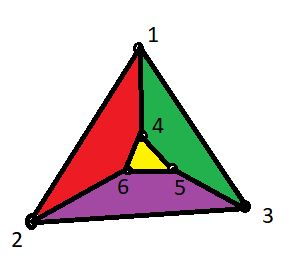
\includegraphics[width=0.5\textwidth]{mapcolor.JPG}
\caption{A graph with four regions or faces, with each region or face colored a different color}\label{10g8}
\end{center}
\end{figure}

Rishnak waved his hands an a new graph appeared, its four faces colored in [Figure~\ref{10g8}]. He said, ``The four faces are~$(1,2,4,6)$, $(1,3,5,4)$, $(2,3,5,6)$ and~$(4,5,6)$. Each of these regions share a border or edge with other regions. Therefore, all of these four regions are mutually adjacent. Often the outside region is also colored. And in this graph, the outside region could be colored yellow just like the center region. We know this because the outside region does not share a border with region~$(4,5,6)$.''

Ajur said, ``So we still need only four colors.''

Rishnak nodded. He said, ``One of the most famous theorems about map coloring is that every planar graph can be map colored with four colors. That is, we need only four colors to color every region such that no two adjacent regions have the same color. Here, have a look at this example map of the USA, colored using only four colors.''

Rishnak waved his hands and a new image appeared in front of Ajur [Figure~\ref{10g9}]. Ajur frowned and said, ``That doesn't look at all like the USA.''

Rishnak laughed and said, ``The regions or faces in this map are indeed the states of the USA, but right, it is not like the normal map of the USA that we see in an atlas. The states are not shaped the same or drawn to scale, but this map of the USA preserves the adjacency relationships between each state. Can you identify the state of Maine?''

\begin{figure}
\begin{center}
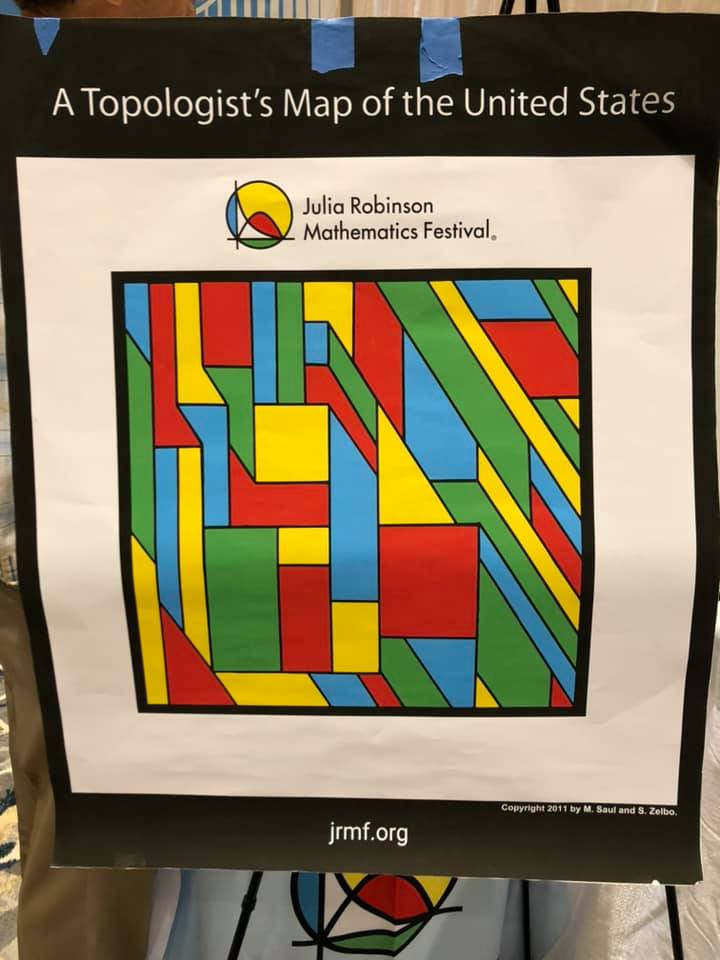
\includegraphics[width=0.5\textwidth]{usamap.png}
\end{center}
\caption{USA Map with face (i.e.,~state) adjacencies preserved, colored using only four colors}\label{10g9}
\end{figure}

Ajur thought for a while, trying to remember how the actual USA map looked. He said, ``I think Maine borders only one other state, New Hampshire. So, the small yellow triangular region in the northeast corner must be the state of Maine.''

Rishnak nodded and said, ``How about the state that borders the most other states? This is actually a tie between two states.''

Ajur raised his eyebrows and said, ``Wow, that's a tough one. They must be states in the Midwest.''

Rishnak said, ``Yes, Tennessee and Missouri both border eight other states. They actually border one another, too.\footnote{Can you find these two states in Figure~\ref{10g9}?} Here's another map, this one of India.''

Rishnak flashed his hands and a map of India with state names shown appeared [Figure~\ref{10g10}]. Rishnak said, ``Could the two states of Andhra Pradesh and Kerala be colored using the same color?''

\begin{figure}
\begin{center}
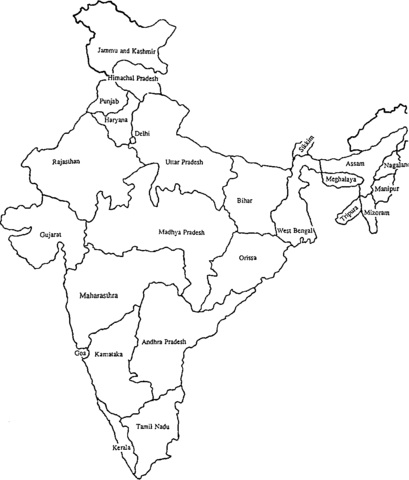
\includegraphics[width=0.9\textwidth]{MapIndia.jpg}
\end{center}
\caption{An old map of India with states and borders shown}\label{10g10}
\end{figure}

Ajur said, ``Yes, they could definitely be colored using the same color because they do not share a border.''

Rishnak asked, ``What about Goa and Kerala?''

Ajur replied instantaneously with a resounding,~``Yes, they also do not share a border. We can just convert the map coloring problem into a vertex coloring problem, similar to converting the edge coloring problem to a vertex coloring problem, right?''

Rishnak said, ``How might you do that?''

Ajur explained that each region or face of the original map would become a vertex of the new graph, and two vertices in the new graph would have an edge to show they are adjacent if the corresponding regions in the original graph shared a border. He said, ``For example, in the map of the USA, all of the states would become vertices of the new graph, with an edge added for each corresponding pair of states that share a border with one another. So the vertex corresponding to Maine would be adjacent only to the vertex corresponding to New Hampshire. Similarly, the vertex corresponding to Washington would be adjacent to vertices corresponding to Oregon and Idaho.''

Rishnak nodded. He was very pleased with the way Ajur was able to quickly absorb the material.

\subsection*{Question for the eighth day}
Rishnak said, ``It is time, Ajur, for the question for the eighth day. Can you color the vertices of this graph''---he flashed his hands to show a new graph [Figure~\ref{colorgq1}]---``with as few colors as possible.''

\textit{Before you turn the page, try to come up with an answer of your own!}

\begin{figure}
\begin{center}
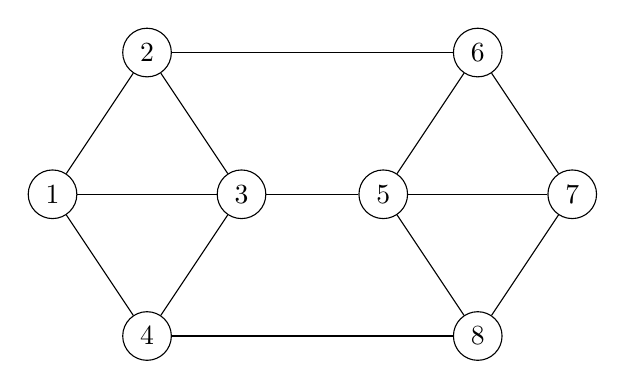
\begin{tikzpicture}
  [scale=.6,auto=left,every node/.style={circle, draw=black}]
  \node (n1) at (0,0) {1};
  \node (n2) at (2,3)  {2};
  \node (n3) at (4,0)  {3};
  \node (n4) at (2,-3) {4};
  \node (n5) at (7,0) {5};
  \node (n6) at (9,3)  {6};
  \node (n7) at (11,0)  {7};
  \node (n8) at (9,-3) {8};

  \foreach \from/\to in {n1/n2,n1/n3,n1/n4,n2/n3,n2/n6, n3/n4, n3/n5, n4/n8, n5/n6,n5/n8,n5/n7,n6/n7,n7/n8}
    \draw (\from) -- (\to);

\end{tikzpicture}

\caption{Can you vertex color this graph with as few colors as possible?}\label{colorgq1}
\end{center}
\end{figure}

\newpage
\subsection*{Answer for the eighth day}
Ajur had no problem coloring this graph as follows Figure \ref{colorga1}

\begin{figure}
\begin{center}
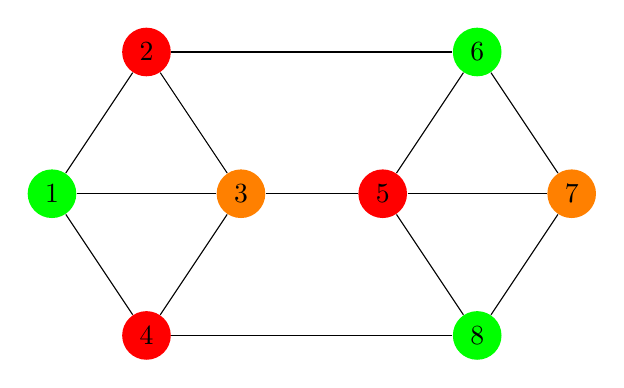
\begin{tikzpicture}
  [scale=.6,auto=left,every node/.style={circle}]
  \node (n1) [fill=green] at (0,0) {1};
  \node (n2) [fill=red] at (2,3)  {2};
  \node (n3) [fill=orange] at (4,0)  {3};
  \node (n4) [fill=red] at (2,-3) {4};
  \node (n5) [fill=red] at (7,0) {5};
  \node (n6) [fill=green] at (9,3)  {6};
  \node (n7) [fill=orange]  at (11,0)  {7};
  \node (n8) [fill=green] at (9,-3) {8};

  \foreach \from/\to in {n1/n2,n1/n3,n1/n4,n2/n3,n2/n6, n3/n4, n3/n5, n4/n8, n5/n6,n5/n8,n5/n7,n6/n7,n7/n8}
    \draw (\from) -- (\to);

\end{tikzpicture}

\caption{Vertex coloring of the graph shown in Figure~\ref{colorgq1} with a minimum number of colors, namely~3}\label{colorga1}
\end{center}
\end{figure}

Rishnak nodded and did not want to push further, so he called it a day. Ajur and Jura walked home, Ajur smiling over everything he had learned that day.
